At most college campuses, as students become more settled within their college community, it becomes increasingly difficult for them to branch out and meet new people beyond their immediate social graph. This is where TA comes in. By providing a way to chat anonymously with (and potentially meet) their fellow classmates, TA allows students to make new connections and shake up their social network. This website also provides a great way to develop and test a new, weakly context-dependent variant of the classic UCB1 multi-armed bandit algorithm (the UCB1-AKSB algorithm, described fully in \autoref{ch:Methods}). The development and performance of UCB1-AKSB is the main focus of this thesis.

\section{What is Tigers Anonymous?}

Tigers Anonymous (TA) is the name of a web application that allows any Princeton student to be matched with another Princeton student. After being matched, the students will be taken to an anonymous chatroom where they are given a conversation starter (an example is shown in \autoref{fig:ConvoStarter}) and have the opportunity to have a conversation. For a complete list of all conversation starters used in TA, see \autoref{app:ConversationStarters}.

Once both participants have exchanged a pre-determined number of messages, a drop-down menu appears containing two choices (see \autoref{fig:DropDownMenu} below). If both users click `Yes', the application will authenticate both users via Facebook and reveal each users' identities to the other to facilitate communication outside of TA. For more information on how TA is implemented, see \autoref{app:TABackendImplementation} and \autoref{app:TAFrontendImplementation}.

\begin{figure}[h]
\centering
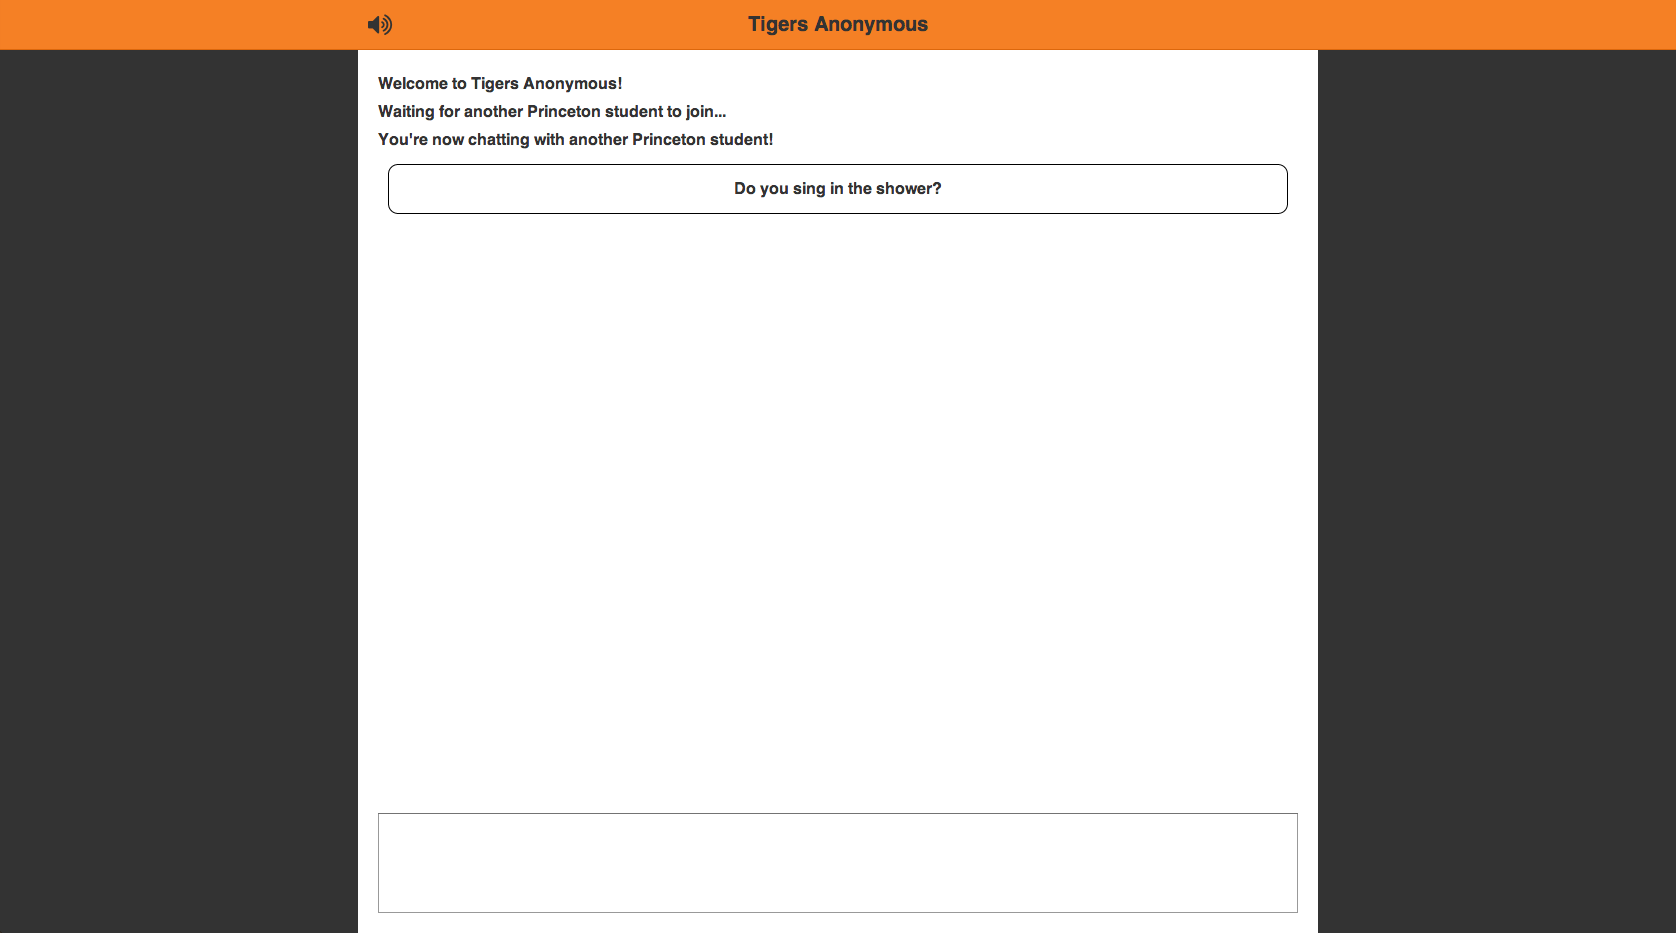
\includegraphics[trim= 120mm 250mm 120mm 0mm, clip, scale=0.36]{./Figures/ConversationStarter}
\caption{TA Conversation Starter}
\label{fig:ConvoStarter}
\end{figure}

\begin{figure}[h]
\centering
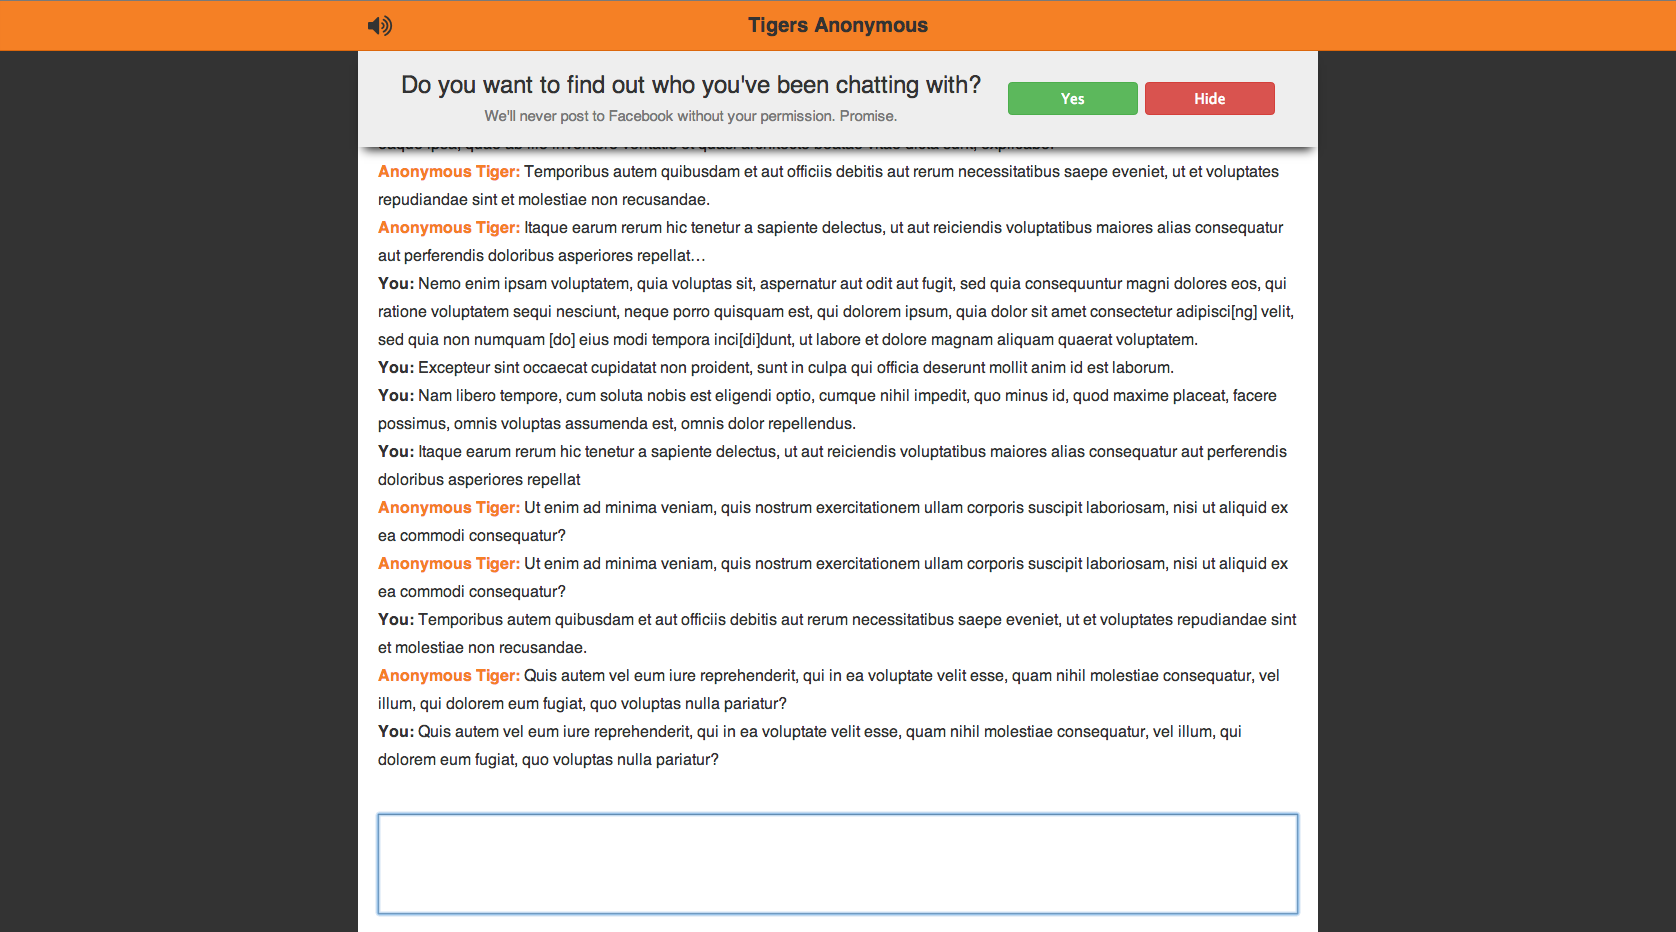
\includegraphics[trim= 120mm 0mm 120mm 0mm, clip, scale=0.36]{./Figures/FullChatDropDown}
\caption{TA Drop-Down Menu}
\label{fig:DropDownMenu}
\end{figure}

\section{Why Multi-Armed Bandits?}
\label{sec:WhyMultiArmedBandits}
A significant part of the functionality of TA is providing a conversation starter to reduce the awkwardness of the initial interaction with an anonymous stranger online. A naive approach would simply choose conversation starters at random, but this approach would be less than optimal for two reasons. First, students might respond better to some conversation starters than others, so TA should be able to select the conversation starters that will facilitate higher quality conversations. Second, users could potentially see the same conversation starter more than once, which would defeat the purpose of having novel conversation starters in the first place.

This is where the multi-armed bandit problem comes in. By modeling conversation starters as `arms' in a classical multi-armed bandit problem and a `success' as a `high-quality' conversation, it should be possible to solve both of the above problems. For more information on the multi-armed bandit problem and the motivation for the UCB1-AKSB algorithm described in \autoref{ch:Methods}, see \autoref{ch:LiteratureReview}.
